\documentclass[border=6pt]{standalone}
\usepackage{newtxtext,newtxmath}
\usepackage{tikz}
\usetikzlibrary{arrows.meta,positioning,shapes.geometric,shapes.misc,calc,fit,backgrounds,automata}
\definecolor{navy}{HTML}{0F294A}
\definecolor{blu}{HTML}{1E56A0}
\definecolor{lblu}{HTML}{EAF1FB}
\definecolor{grn}{HTML}{1E8449}
\definecolor{lgrn}{HTML}{E9F7EF}
\definecolor{org}{HTML}{CA6F1E}
\definecolor{lorg}{HTML}{FDF2E9}
\definecolor{red}{HTML}{B03A2E}
\definecolor{lred}{HTML}{FDEDEC}
\definecolor{pur}{HTML}{7D3C98}
\definecolor{lpur}{HTML}{F4ECF7}
\definecolor{gry}{HTML}{5D6D7E}
\definecolor{lgry}{HTML}{F4F6F7}
\tikzset{
  >={Stealth[length=2.6mm,width=1.9mm]},
  every node/.style={font=\small},
  blk/.style={draw=blu, fill=lblu, rounded corners=2pt, line width=0.7pt, align=center,
              minimum height=10mm, text width=#1, inner sep=3pt},
  blk/.default=30mm,
  flow/.style={->, line width=0.8pt, draw=navy},
  lbl/.style={font=\footnotesize\itshape, text=navy},
  frame/.style={draw=#1, dashed, rounded corners=4pt, line width=0.9pt, inner sep=7pt},
  ttl/.style={font=\small\bfseries, text=#1},
}

\begin{document}
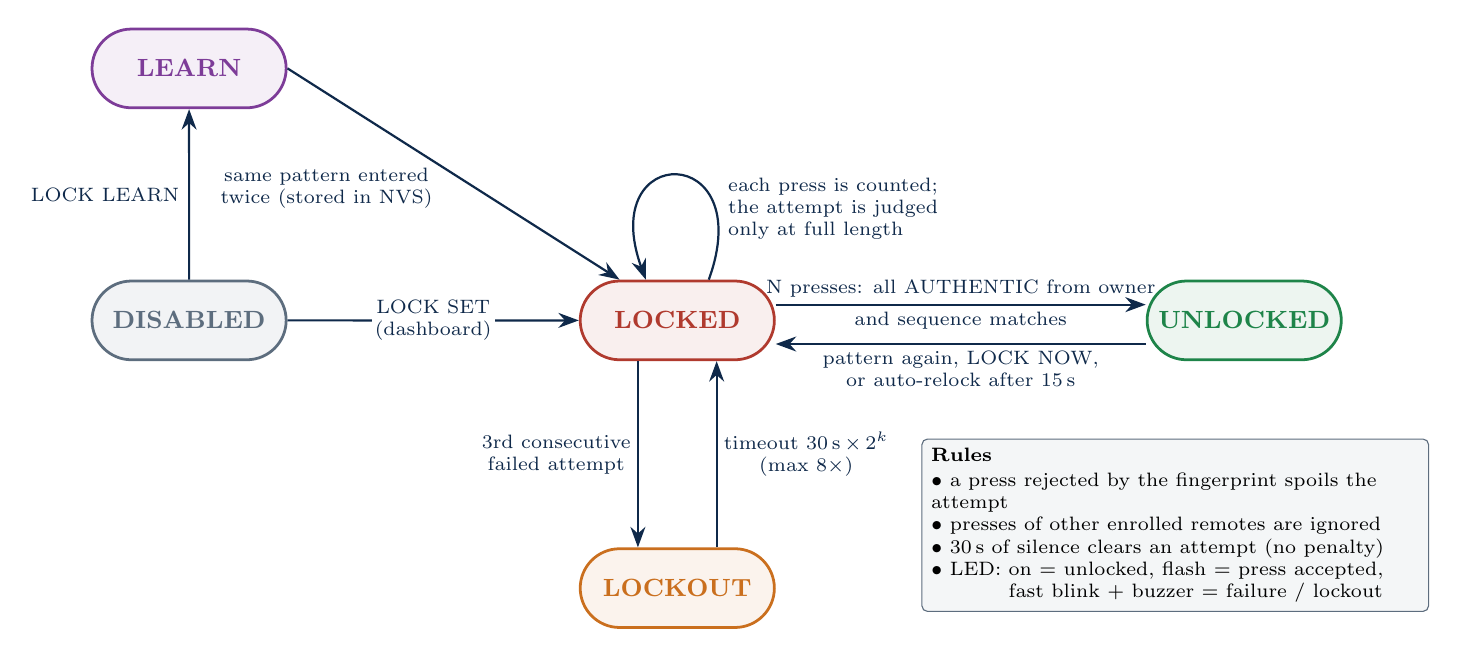
\begin{tikzpicture}[every node/.style={font=\footnotesize}]
\tikzset{
 st/.style={rounded rectangle, draw=#1, line width=1pt, fill=#1!8, minimum width=27mm, minimum height=10mm, font=\small\bfseries, text=#1},
 tr/.style={->, line width=0.8pt, draw=navy},
 tl/.style={font=\scriptsize, text=navy, align=center, fill=white, inner sep=1.2pt},
}
\node[st=gry] (dis) at (0,0) {DISABLED};
\node[st=pur] (lrn) at (0,3.2) {LEARN};
\node[st=red] (lck) at (6.2,0) {LOCKED};
\node[st=grn] (unl) at (13.4,0) {UNLOCKED};
\node[st=org] (out) at (6.2,-3.4) {LOCKOUT};
\draw[tr] (dis) -- node[tl, left=2pt, fill=none] {LOCK LEARN} (lrn);
\draw[tr] (lrn.east) -- node[tl, pos=0.45, below left=0pt and 0pt, fill=none] {same pattern entered\\twice (stored in NVS)} (lck.north west);
\draw[tr] (dis) -- node[tl] {LOCK SET\\(dashboard)} (lck);
\draw[tr] ([yshift=2mm]lck.east) -- node[tl, above=1pt, fill=none] {N presses: all AUTHENTIC from owner}
                                      node[tl, below=1pt, fill=none] {and sequence matches} ([yshift=2mm]unl.west);
\draw[tr] ([yshift=-3mm]unl.west) -- node[tl, below=1pt, fill=none, align=center] {pattern again, LOCK NOW,\\or auto-relock after 15\,s} ([yshift=-3mm]lck.east);
\draw[tr] ([xshift=-5mm]lck.south) -- node[tl, left=1pt, fill=none] {3rd consecutive\\failed attempt} ([xshift=-5mm]out.north);
\draw[tr] ([xshift=5mm]out.north) -- node[tl, right=1pt, fill=none] {timeout 30\,s\,$\times\,2^{k}$\\(max $8\times$)} ([xshift=5mm]lck.south);
\draw[tr] ([xshift=4mm]lck.north) to[out=70, in=110, looseness=6] node[tl, pos=0.22, right=3pt, fill=none, align=left] {each press is counted;\\the attempt is judged\\only at full length} ([xshift=-4mm]lck.north);
\node[draw=gry, fill=lgry, rounded corners=2pt, align=left, text width=62mm, font=\scriptsize, anchor=north west] at (9.3,-1.5)
 {\textbf{Rules}\\[1pt]
  $\bullet$ a press rejected by the fingerprint spoils the attempt\\
  $\bullet$ presses of other enrolled remotes are ignored\\
  $\bullet$ 30\,s of silence clears an attempt (no penalty)\\
  $\bullet$ LED: on = unlocked, flash = press accepted,\\\phantom{$\bullet$ LED: }fast blink + buzzer = failure / lockout};
\end{tikzpicture}
\end{document}
